\documentclass[12pt]{article}
\usepackage[utf8]{inputenc}
\usepackage[english]{babel}
\usepackage[letterpaper, portrait, margin=1in]{geometry}
\usepackage{amsmath}
\numberwithin{equation}{section}
\usepackage{amssymb}
\usepackage{graphicx}
\usepackage{parskip}
\usepackage{xcolor}
\usepackage{physics}
\usepackage{empheq}
\usepackage{cancel}
\usepackage{hyperref}
\hypersetup{colorlinks = true, urlcolor = blue, linkcolor = red, citecolor = red}
\usepackage{enumerate}
\usepackage{tikz}
\usepackage{float}
\usepackage{tcolorbox}
\usepackage{booktabs}
\usepackage[bottom]{footmisc}

% Default fixed font does not support bold face
\DeclareFixedFont{\ttb}{T1}{txtt}{bx}{n}{12} % for bold
\DeclareFixedFont{\ttm}{T1}{txtt}{m}{n}{12}  % for normal

% Custom colors
\usepackage{color}
\definecolor{deepblue}{rgb}{0,0,0.5}
\definecolor{deepred}{rgb}{0.6,0,0}
\definecolor{deepgreen}{rgb}{0,0.5,0}

\usepackage{listings}

% Python style for highlighting
\newcommand\pythonstyle{\lstset{
		language=Python,
		basicstyle=\ttm,
		morekeywords={self},              % Add keywords here
		commentstyle=\color{gray},
		keywordstyle=\ttb\color{deepblue},
		emph={MyClass,__init__},          % Custom highlighting
		emphstyle=\ttb\color{deepred},    % Custom highlighting style
		stringstyle=\color{deepgreen},                        % Any extra options here
		showstringspaces=false
}}


% Python environment
\lstnewenvironment{python}[1][]
{
	\pythonstyle
	\lstset{#1}
}
{}

% Python for external files
\newcommand\pythonexternal[2][]{{
		\pythonstyle
		\lstinputlisting[#1]{#2}}}

% Python for inline
\newcommand\pythoninline[1]{{\pythonstyle\lstinline!#1!}}

\usepackage{xcolor}
\usepackage{fancyhdr}
\pagestyle{fancy}
\fancyhf{}
\fancyfoot[C]{\color{lightgray} Statistics Lecture II Notes}
\fancyfoot[L]{\color{lightgray} \today}
\fancyfoot[R]{Page \thepage}
\renewcommand{\headrulewidth}{0pt}
\renewcommand{\footrulewidth}{0pt}

\begin{document}
	
\section{Introduction}
\begin{itemize}
	\item Today we will discuss curve fitting.
	\item (1) the least squares method, (2) implementing least squares with Scipy, (3) $ \chi^2 $ analysis of goodness-of-fit (how well our model actually describes the data).
\end{itemize}

\section{Least Squares Regression}
\begin{itemize}
\item VARIABLES: when we collect data, we vary and independent variable(s) $ x_i $ and observe the dependent variable $ y_i $. The data that we collect is of the form: 
\begin{equation}
		\{(x_1, y_1),(x_2, y_2),\dots, (x_m, y_m) \}
\end{equation}
\item MODEL: a description of how we expect $ y_i $  to relate to $ x_i $ with parameters,
\begin{equation}
		\lambda_1,\lambda_2,\dots,\lambda_n = \vec{\lambda};\quad m>n
\end{equation}
We write the model as,
\begin{equation}
		f(\vec{\lambda};x)
\end{equation}
We FIT our data to the model by finding the values of $ \vec{\lambda} $ so that $ \hat{y}_i = f(\vec{\lambda};x) $ matches $ y_i $ as close as possible.

\item We say the model is LINEAR if $ f(\vec{\lambda};x) $ is linear in $ \vec{\lambda} $,
\begin{equation}
		f(a\vec{\lambda}_0+b\vec{\lambda}_1;x) = a f(\vec{\lambda}_0;x) + bf(\vec{\lambda}_1;x) 
\end{equation}
If $ f(\vec{\lambda};x) $ is linear, then,
\begin{equation}
		f(\vec{\lambda};x) = \sum_{j=0}^n \lambda_j \cdot f_j(x);\quad \text{where }f_j(x) \text{ are arbitrary functions}
\end{equation}
Examples:
\begin{enumerate}
	\item $  f(\vec{\lambda};x) = \lambda_0 + \lambda_1 x + \lambda_2 x^2 $
	\item $ f(\vec{\lambda};x) = \lambda_0 x+ \lambda_1 \sin(x) $
	\item $ f(\vec{\lambda};x) = \lambda_0 \sin(x)+ \lambda_1 \sin(x) $
\end{enumerate}
\item A model is NONLINEAR if $ f(\vec{\lambda};x) $ is not linear in $ \vec{\lambda} $,
Examples:
\begin{enumerate}
	\item $ \sin(\lambda_0 x + \lambda_1x)  $
	\item $ \lambda_0 x/(\lambda_1 + x) $
\end{enumerate}
\item LEAST SQUARES: how do we know when the parameters $ \vec{\lambda} $ have been optimized? We define our heuristic $ \phi $ as the sum of the square residues,
\begin{equation}
		\boxed{\phi = \sum_{i=0}^m r_i^2 = \sum_{i=0}^m [y_i - f(\vec{\lambda};x_i)]^2}
\end{equation}
[Draw picture of residues]

Least squares regression is the task of minimizing $ \phi $. When $ \phi $ is minimum,
\begin{equation}
		\grad_{\vec{\lambda}}\  \phi = 0
\end{equation}
(the subscript $ \vec{\lambda} $ means we are taking the partial derivative w.r.t. the parameters $ \vec{\lambda} $.)

$ \phi $ is a complicated function, computing it's gradient and finding the values of $ \vec{\lambda} $ that make the gradient zero is not an easy task!
\begin{enumerate}
	\item An exact solution for $ \vec{\lambda} $ can be determined in the linear least squares case with some vector calculus (perhaps with some caveats I don't know of...I'm not a statistician)
	\item There is no exact, general solution for the nonlienar least squares case. Instead, we use numerical techniques to APPROXIMATE solutions.
	\item In practice: we will use an exact solution for the line, and use numerical fittings for all other cases (linear and nonlinear).
\end{enumerate}

NOTE: $ \grad_{\vec{\lambda}}\  \phi = 0 $ only gives us the critical points. To be rigorous, we should show that the critical points are indeed minimum. In practice, we shall be a bit lazy and omit this step.

\end{itemize}

\subsection{Least squares regression for a line}
\begin{itemize}
\item We will use the model,
\begin{equation}
		f(\vec{\lambda}; x) = \lambda_0 + \lambda_1 x
\end{equation}
where $ \lambda_0 $ is the y-intercept and $ \lambda_1 $ is the slope.
\item Minimizing $ \phi $,
\begin{align}
	0 &= \grad_{\vec{\lambda}}\  \phi  = \grad_{\vec{\lambda}}\  \sum_{i=0}^m [y_i - f(\vec{\lambda};x_i)]^2 = \grad_{\vec{\lambda}}\  \sum_{i=0}^m [y_i - \lambda_0 - \lambda_1 x_i]^2\\
	&= \pdv{}{\lambda_0} \sum_{i=0}^m [y_i - \lambda_0 - \lambda_1 x_i]^2 \label{eq:1}\\
	&= \pdv{}{\lambda_1} \sum_{i=0}^m [y_i - \lambda_0 - \lambda_1 x_i]^2 \label{eq:2}
\end{align}

\item First component (\ref{eq:1})
\begin{align*}
	0 &= \pdv{}{\lambda_0} \sum_{i=0}^m [y_i - \lambda_0 - \lambda_1 x_i]^2 \\
	&= \pdv{}{\lambda_0} \sum_{i=0}^m [y_i^2 - \lambda_0 y_i - \lambda_1x_iy_i - \lambda_0y_i + \lambda_0^2 + \lambda_0\lambda_1x_i - \lambda_1x_iy_i + \lambda_0\lambda_1x_i + \lambda_1^2x_i^2]\\
	&=  \sum_{i=0}^m \pdv{}{\lambda_0} [y_i^2 - 2\lambda_0y_i - 2\lambda_1x_iy_i + \lambda_0^2 + 2\lambda_0\lambda_1x_i + \lambda_1^2x_i^2]\\
	&=  \sum_{i=0}^m (-2y_i + 2\lambda_0 + 2\lambda_1x_i)=  \sum_{i=0}^m y_i - \lambda_0 - \lambda_1x_i)\\
	&=\left(\sum_{i=0}^m y_i\right) - m\lambda_0 - b\left(\sum_{i=0}^m x_i\right) \\
\end{align*}
\begin{equation}
			\lambda_0 = \frac{\left(\sum_i y_i\right) - b\left(\sum_i x_i\right)}{m} = \bar{y} - \lambda_1\bar{x}
\end{equation}

\item Second component (\ref{eq:2})
\begin{align*}
	0 &= \pdv{}{\lambda_1} \sum_{i=0}^m [y_i - \lambda_0 - \lambda_1 x_i]^2 \\
	&=  \sum_{i=0}^m\pdv{}{\lambda_1} [y_i^2 - 2\lambda_0y_i - 2\lambda_1x_iy_i + \lambda_0^2 + 2\lambda_0\lambda_1x_i + \lambda_1^2x_i^2]\\
	&= \sum_{i=0}^m(-2x_iy_i + 2\lambda_0x_i + 2\lambda_1x_i^2)= \sum_{i=0}^m (\lambda_1x_i^2 + \lambda_0x_i - x_iy_i)\\
	& = \sum_{i=0}^m (\lambda_1x_i^2 + (\bar{y} - \lambda_1\bar{x})x_i - x_iy_i)= \sum_{i=0}^m (\lambda_1x_i^2 + x_i\bar{y} - \lambda_1x_i\bar{x} - x_iy_i)\\
	&= \lambda_1\ \sum_i(x_i^2 - x_i\bar{x}) + \sum_i (x_i\bar{x} - x_iy_i)\\
\end{align*}
We will need below that: $ \sum_i (\bar{x}^2 - x_i\bar{x})  = \sum_i (\bar{x}\bar{y} - y_i\bar{x}) = 0$
\begin{align*}
		\lambda_1 &= \frac{\sum_i (x_iy_i - x_i\bar{x} )}{\sum_i(x_i^2 - x_i\bar{x})} =  \frac{\sum_i (x_iy_i - x_i\bar{x} ) + \sum_i (\bar{x}\bar{y} - y_i\bar{x}) }{\sum_i(x_i^2 - x_i\bar{x}) + \sum_i (\bar{x}^2 - x_i\bar{x}) } \\
		&= \frac{\frac{1}{m} \sum_i (x_i-\bar{x})(y_i-\bar{y})}{\frac{1}{m} \sum_i (x_i-\bar{x})^2} = \frac{Cov(x,y)}{Var(x)}
\end{align*}

\begin{equation}
		\boxed{\lambda_1 =\frac{Cov(x,y)}{Var(x)};\quad \lambda_0 =  \bar{y} - \lambda_1\bar{x} }
\end{equation}

\end{itemize}

\subsection{Gauss-Newton method for nonlinear least squares [Optional]}
\begin{itemize}
	\item This is an approximate least squares method for a general nonlinear regression $ f(\vec{\lambda}; x) $. Recall that the goal of the least squares method is to minimize,
	\begin{equation}
			\phi = \sum_i [y_i - f(\vec{\lambda};x_i)]^2
	\end{equation}
	\item Recall Newton's method: a method to approximate the roots of a function $ f(x) $.
\begin{enumerate}
	\item We make an initial guess for the root $ x_0 $
	\item We approximate the function at $ x_0 $ as a line, and define the next approximation $ x_1 $ as the zero of the line
	\begin{align}
			y(x) &= f'(x_0)(x-x_0) + f(x_0)\\
			0 &= f'(x_0)(x_1-x_0) + f(x_0)
	\end{align}
	\begin{equation}
			x_1 = x_0 - f(x_0)/f'(x_0)
	\end{equation}
Generalizing,
\begin{equation}
			x_{k+1} = x_k -  \frac{f(x_k)}{f'(x_k)}
\end{equation}
\end{enumerate}
\item We can use Newton's method to approximate the root of  $ \grad_{\vec{\lambda}}\  \phi $ [NOTE: it is implied that all further derivatives are w.r.t $\vec{\lambda}$, so I will omit the subscript moving forward. In particular, the $ \laplacian $ is not the Laplacian, but is really the Hessian $ \laplacian_{\vec{\lambda}} = H $],
\begin{equation}
		\vec{\lambda}_{k+1} = 	\vec{\lambda}_{k} - \frac{\grad\phi(\vec{\lambda}_k)}{\laplacian\phi(\vec{\lambda}_k)} 
\end{equation}
\item Before we find an expression for $ \vec{\lambda}_{k+1}  $, recall the JACOBIAN is the generalization of the derivative operator to vector-valued functions. For the vector-valued function $ \mathbf{f}(\vec{\lambda}_k) = \left(f(\vec{\lambda}_k; x_1), f(\vec{\lambda}_k; x_2), \dots, f(\vec{\lambda}_k; k_n)\right)^T$,
\begin{equation}
		 \mathbf {J} ={\begin{pmatrix}\nabla ^{\mathrm {T} }f_{1}\\\vdots \\\nabla ^{\mathrm {T} }f_{m}\end{pmatrix}}={\begin{pmatrix}{\dfrac {\partial f_{1}}{\partial \lambda_{1}}}&\cdots &{\dfrac {\partial f_{1}}{\partial \lambda_{n}}}\\   \dfrac {\partial f_{2}}{\partial \lambda_{1}}  & \cdots & \dfrac {\partial f_{2}}{\partial \lambda_{n}} \\\vdots &\ddots &\vdots \\{\dfrac {\partial f_{m}}{\partial \lambda_{1}}}&\cdots &{\dfrac {\partial f_{m}}{\partial \lambda_{n}}}\end{pmatrix}}
\end{equation}

\item The GRADIENT. Examining a single component,
\begin{equation}
		\left(\grad{\phi(\vec{\lambda}_k)}\right)_j = \pdv{}{\lambda_j}\sum_i [y_i - f(\vec{\lambda}_k;x_i)]^2 = \sum_i -2[y_i - f(\vec{\lambda}_k;x_i)]\pdv{f(\vec{\lambda}_k; x_i)}{\lambda_j} 
\end{equation}
Therefore,
\begin{equation}
		\grad{\phi(\vec{\lambda}_k)} = -2\,\mathbf{J}^T \mathbf{r}
\end{equation}
where $ \mathbf{r}$ is the vector of residuals, $ r_i =  y_i - f(\vec{\lambda}_k;x_i)$. NOTICE: $ \mathbf{J} $ and $ \mathbf{r} $ are both functions of $ \vec{\lambda_k} $.
\item The HESSIAN (what is the Hessian? See \href{https://najeebkhan.github.io/blog/VecCal.html}{\textit{Gradient, Jacobian, Hessian, Laplacian and all that}}). Examining a single component,
\begin{align*}
		H_{l,m} &= \laplacian_{\lambda_l,\lambda_m} {\phi(\vec{\lambda}_k)} = \pdv{\lambda_l}\pdv{\lambda_m}\sum_i [y_i - f(\vec{\lambda}_k;x_i)]^2 \\
		&=  \pdv{\lambda_l} \sum_i -2[y_i - f(\vec{\lambda}_k;x_i)]\pdv{f(\vec{\lambda}_k; x_i)}{\lambda_m} \\
		&= -2\sum_i \left(-\pdv{f(\vec{\lambda}_k; x_i)}{\lambda_l}\pdv{f(\vec{\lambda}_k; x_i)}{\lambda_m} + r_i\pdv{f(\vec{\lambda}_k; x_i)}{\lambda_l}{\lambda_m} \right)\\
		& \approx  2\sum_i \pdv{f(\vec{\lambda}_k; x_i)}{\lambda_l}\pdv{f(\vec{\lambda}_k; x_i)}{\lambda_m} 
\end{align*}
Therefore,
\begin{equation}
		\laplacian{\phi(\vec{\lambda}_k)}= 2\mathbf{J}^T \mathbf{J}
\end{equation}
\item Putting everything together,
\begin{equation}
			\vec{\lambda}_{k+1} = 	\vec{\lambda}_{k} - (\mathbf{J}_k^T \mathbf{J}_k)^{-1}\mathbf{J}_k^T\mathbf{r}
\end{equation}
When implementing this algorithm, we can determine $ \mathbf{J}_k $ numerically (i.e. estimating the derivatives about $ \vec{\lambda}_k $). 

NOTICE: this procedure is sensitive to the initial condition $ \vec{\lambda}_0 $. The successive approximation is not guaranteed to converge, and if it does, it is not guaranteed to be the absolute minimum. Rather, different initial conditions may lead to different local minimums.

\end{itemize}

\section{curve\_fit with scipy.optimize}
\begin{itemize}
\item In our discussion of the Gauss-Newton method, we saw that the solution to the least squares method can be numerically approximated. This is what often happens in practice, and is what we commonly mean by curve fitting.
\item The package scipy has the function \verb|scipy.optimize.curve_fit| which performs a least squares regression using the Levenberg-Marquardt algorithm This algorithm is similar to the Gauss-Newton method, with a few modifications that make it a bit more robust.
\item First, let's create define our model, a line in this case,
\begin{python}
def f(x, a, b):
	'''
	Parameters
		x: ndarray of x-values
		a: slope
		b: intercept
	
	Returns: ndarray of line
	'''
	return a*x + b
	
# plot
x = np.linspace(0,10,100)
y = f(x, 1, 5)
plt.plot(x,y)
plt.show()
\end{python}
\item Generate some random data,
\begin{python}
n = 20
x = np.linspace(0,10,n)
y = 2*x + 3 + np.random.normal(scale=3, size=n)
plt.plot(x,y,'.')
plt.show()
\end{python}

\item Least squares regression with \verb|curve_fit|
\begin{figure}[H]
	\centering
	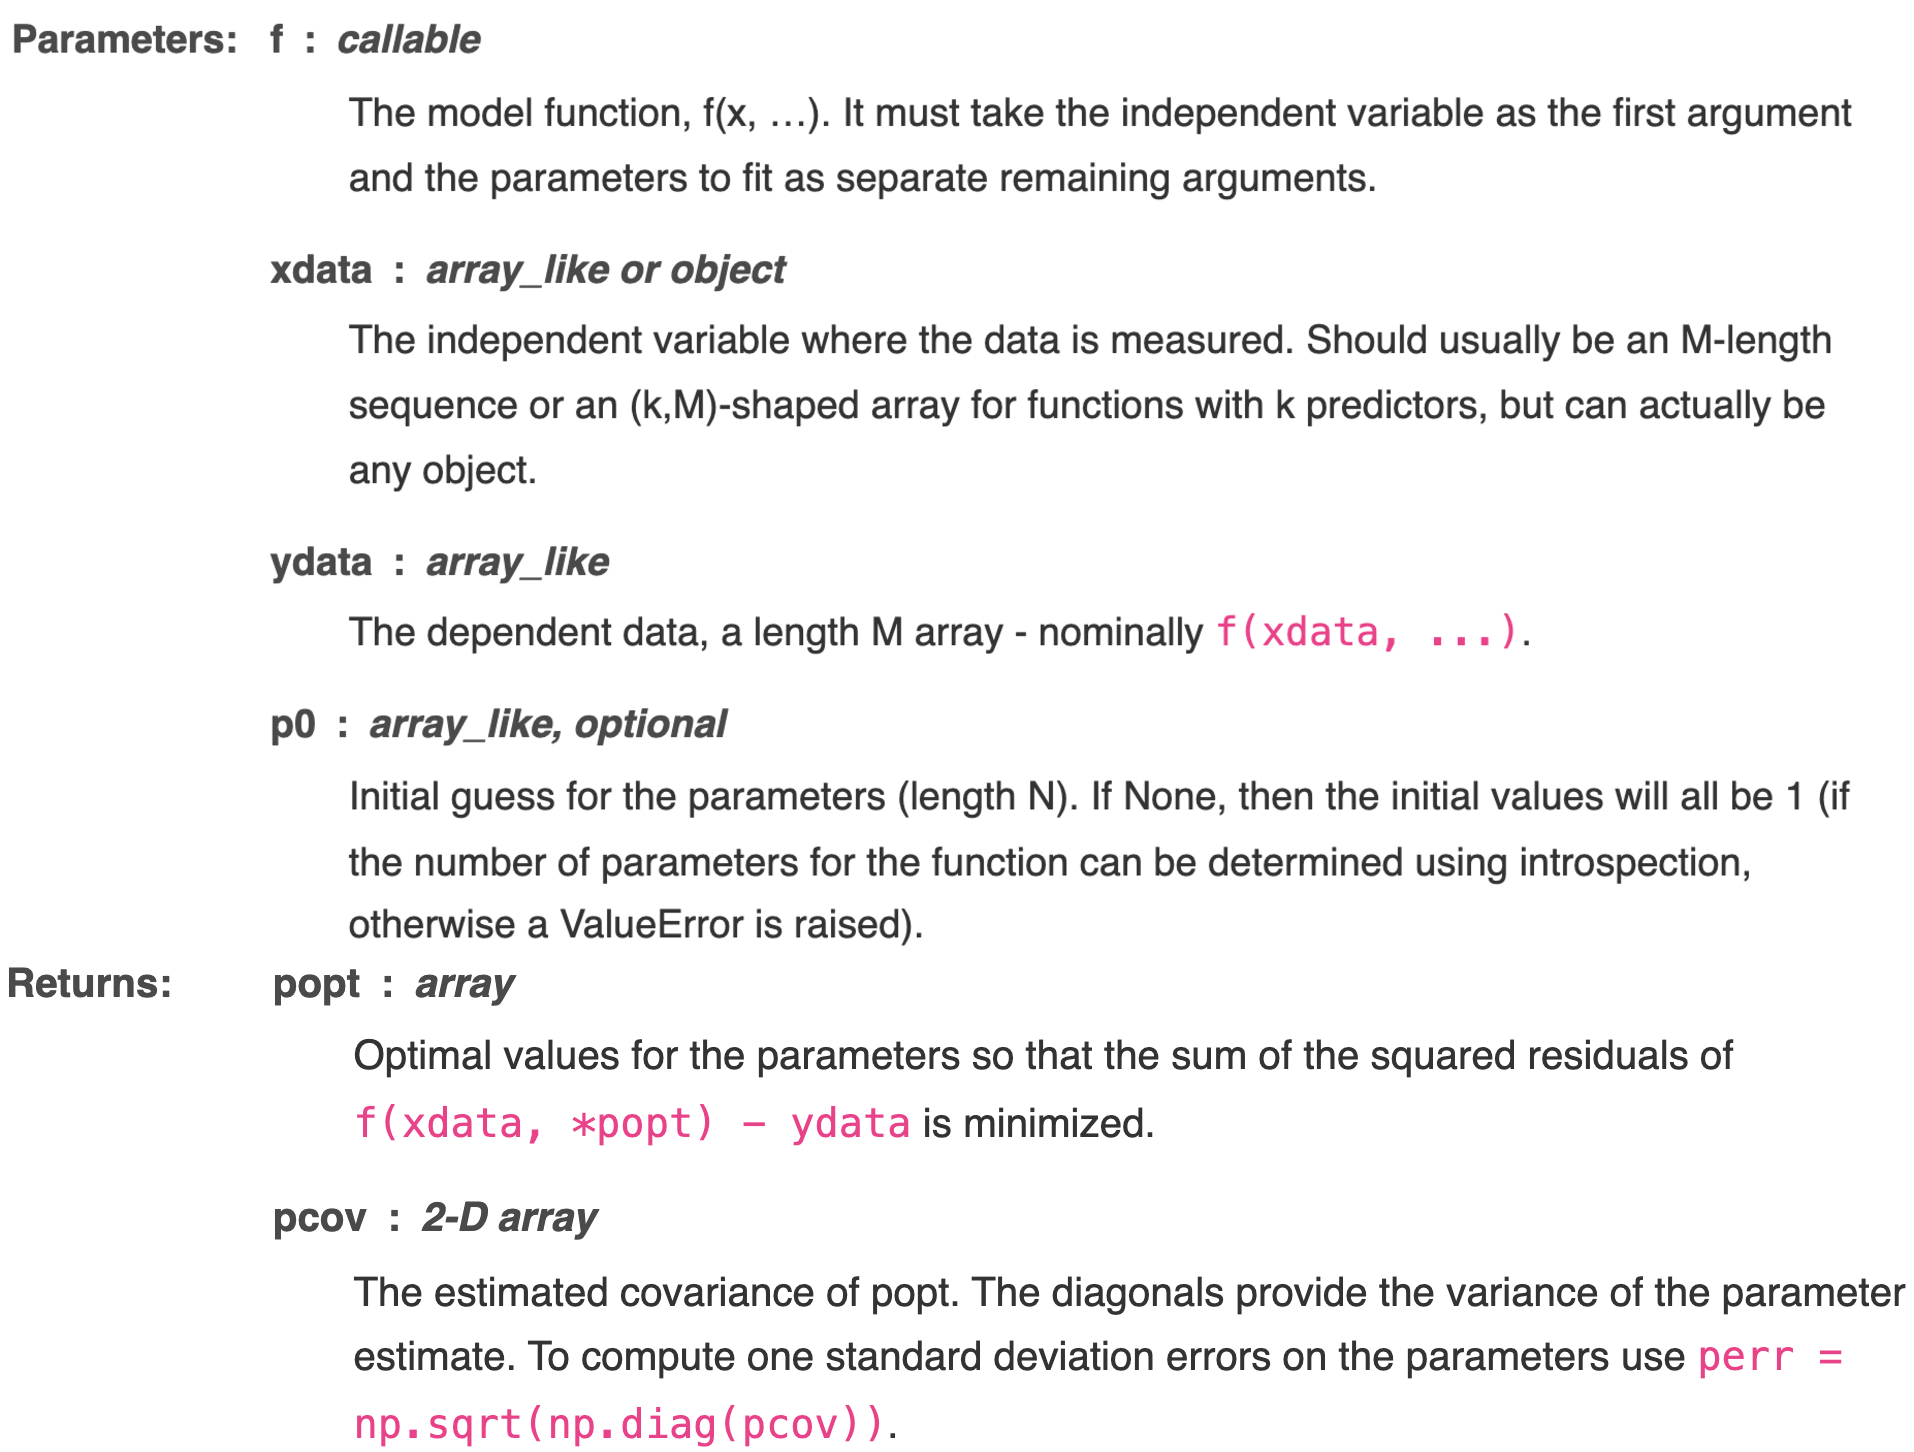
\includegraphics[width=12cm] {cf}
\end{figure}
\begin{python}
popt, pcov = curve_fit(f, x, y)
perr = np.sqrt(np.diag(pcov))

label = f'a={popt[0]:.2f}$\pm${perr[0]:.2f}'
label += f'\nb={popt[1]:.2f}$\pm${perr[1]:.2f}'

fig, ax = plt.subplots()
ax.plot(x,y,'.', label='data')
ax.plot(x, f(x,*popt), label=label)
ax.legend()
plt.show()
\end{python}

\end{itemize}

\section{$\chi^2$ Goodness-of-fit}
\begin{itemize}
\item For a more thorough treatment of this topic: \href{https://www.ocf.berkeley.edu/~yizhu/static/notes/Chi%20Squared/chi_squared.pdf}{link}
\item How do we know our model is correct and that we have a good fit? \textit{Can't we just look at the sum of the square residuals? If it's a small value, then the fit must be good.} NO! For example, we can have the wrong model, but still have small residuals, 
\begin{figure}[H]
	\centering
	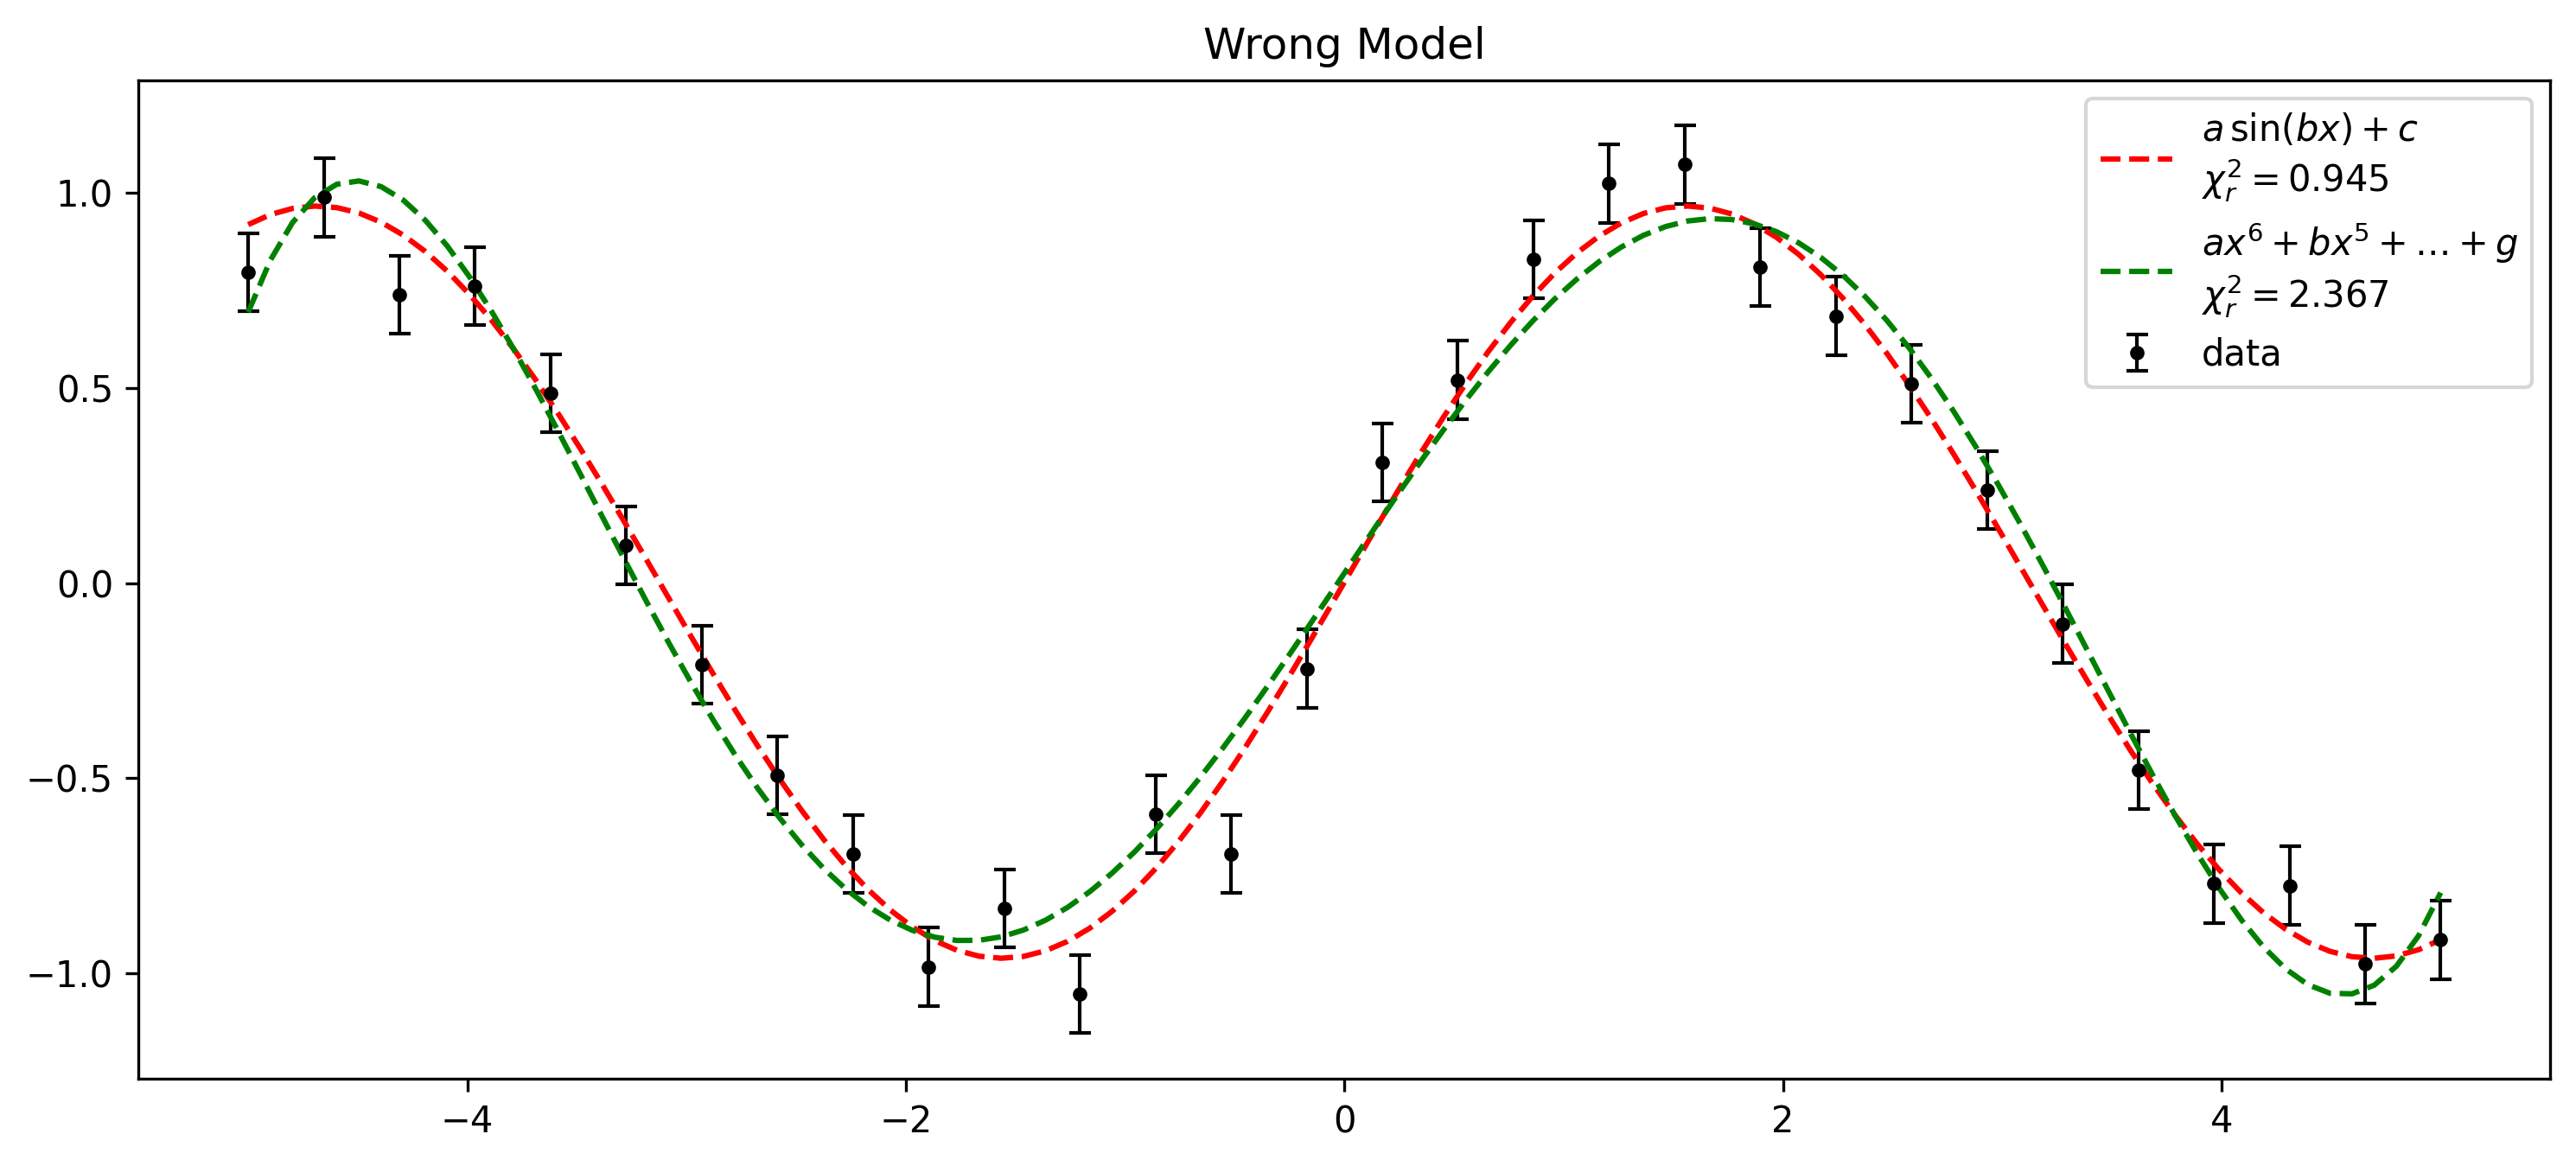
\includegraphics[width=15cm] {wrong}
\end{figure}
The data points are generated by adding normal noise to a sin curve. Both a sin and an order-6 polynomial provide a good fit (by inspection). But the incorrect polynomial fit has a reduced $ \chi^2 >1$, indicating something is off!

So what is this REDUCED CHI-SQUARED?

\item CHI-SQUARED DISTRIBUTION: suppose $X_1, X_2, \dots, X_k$ are $k$ i.i.d. standard normal distributions $X_i\sim N(0,1)$. We define the chi-squared distribution with $k$ degrees of freedom as the sum of the squared $X_i$ distributions,
\begin{equation}
	\chi^2_k = \sum_{i=1}^{k} X_i^2
\end{equation}
The chi-squared distribution has probability density function (derivation \href{https://www.ocf.berkeley.edu/~yizhu/static/notes/Chi%20Squared/chi_squared.pdf}{here}),
\begin{equation}
	f_{\chi^2_k}(x) = \frac{e^{-x/2}\ x^{(k/2-1)}}{2^{k/2}\ \Gamma(k/2)} 
\end{equation}
\begin{figure}[H]
	\centering
	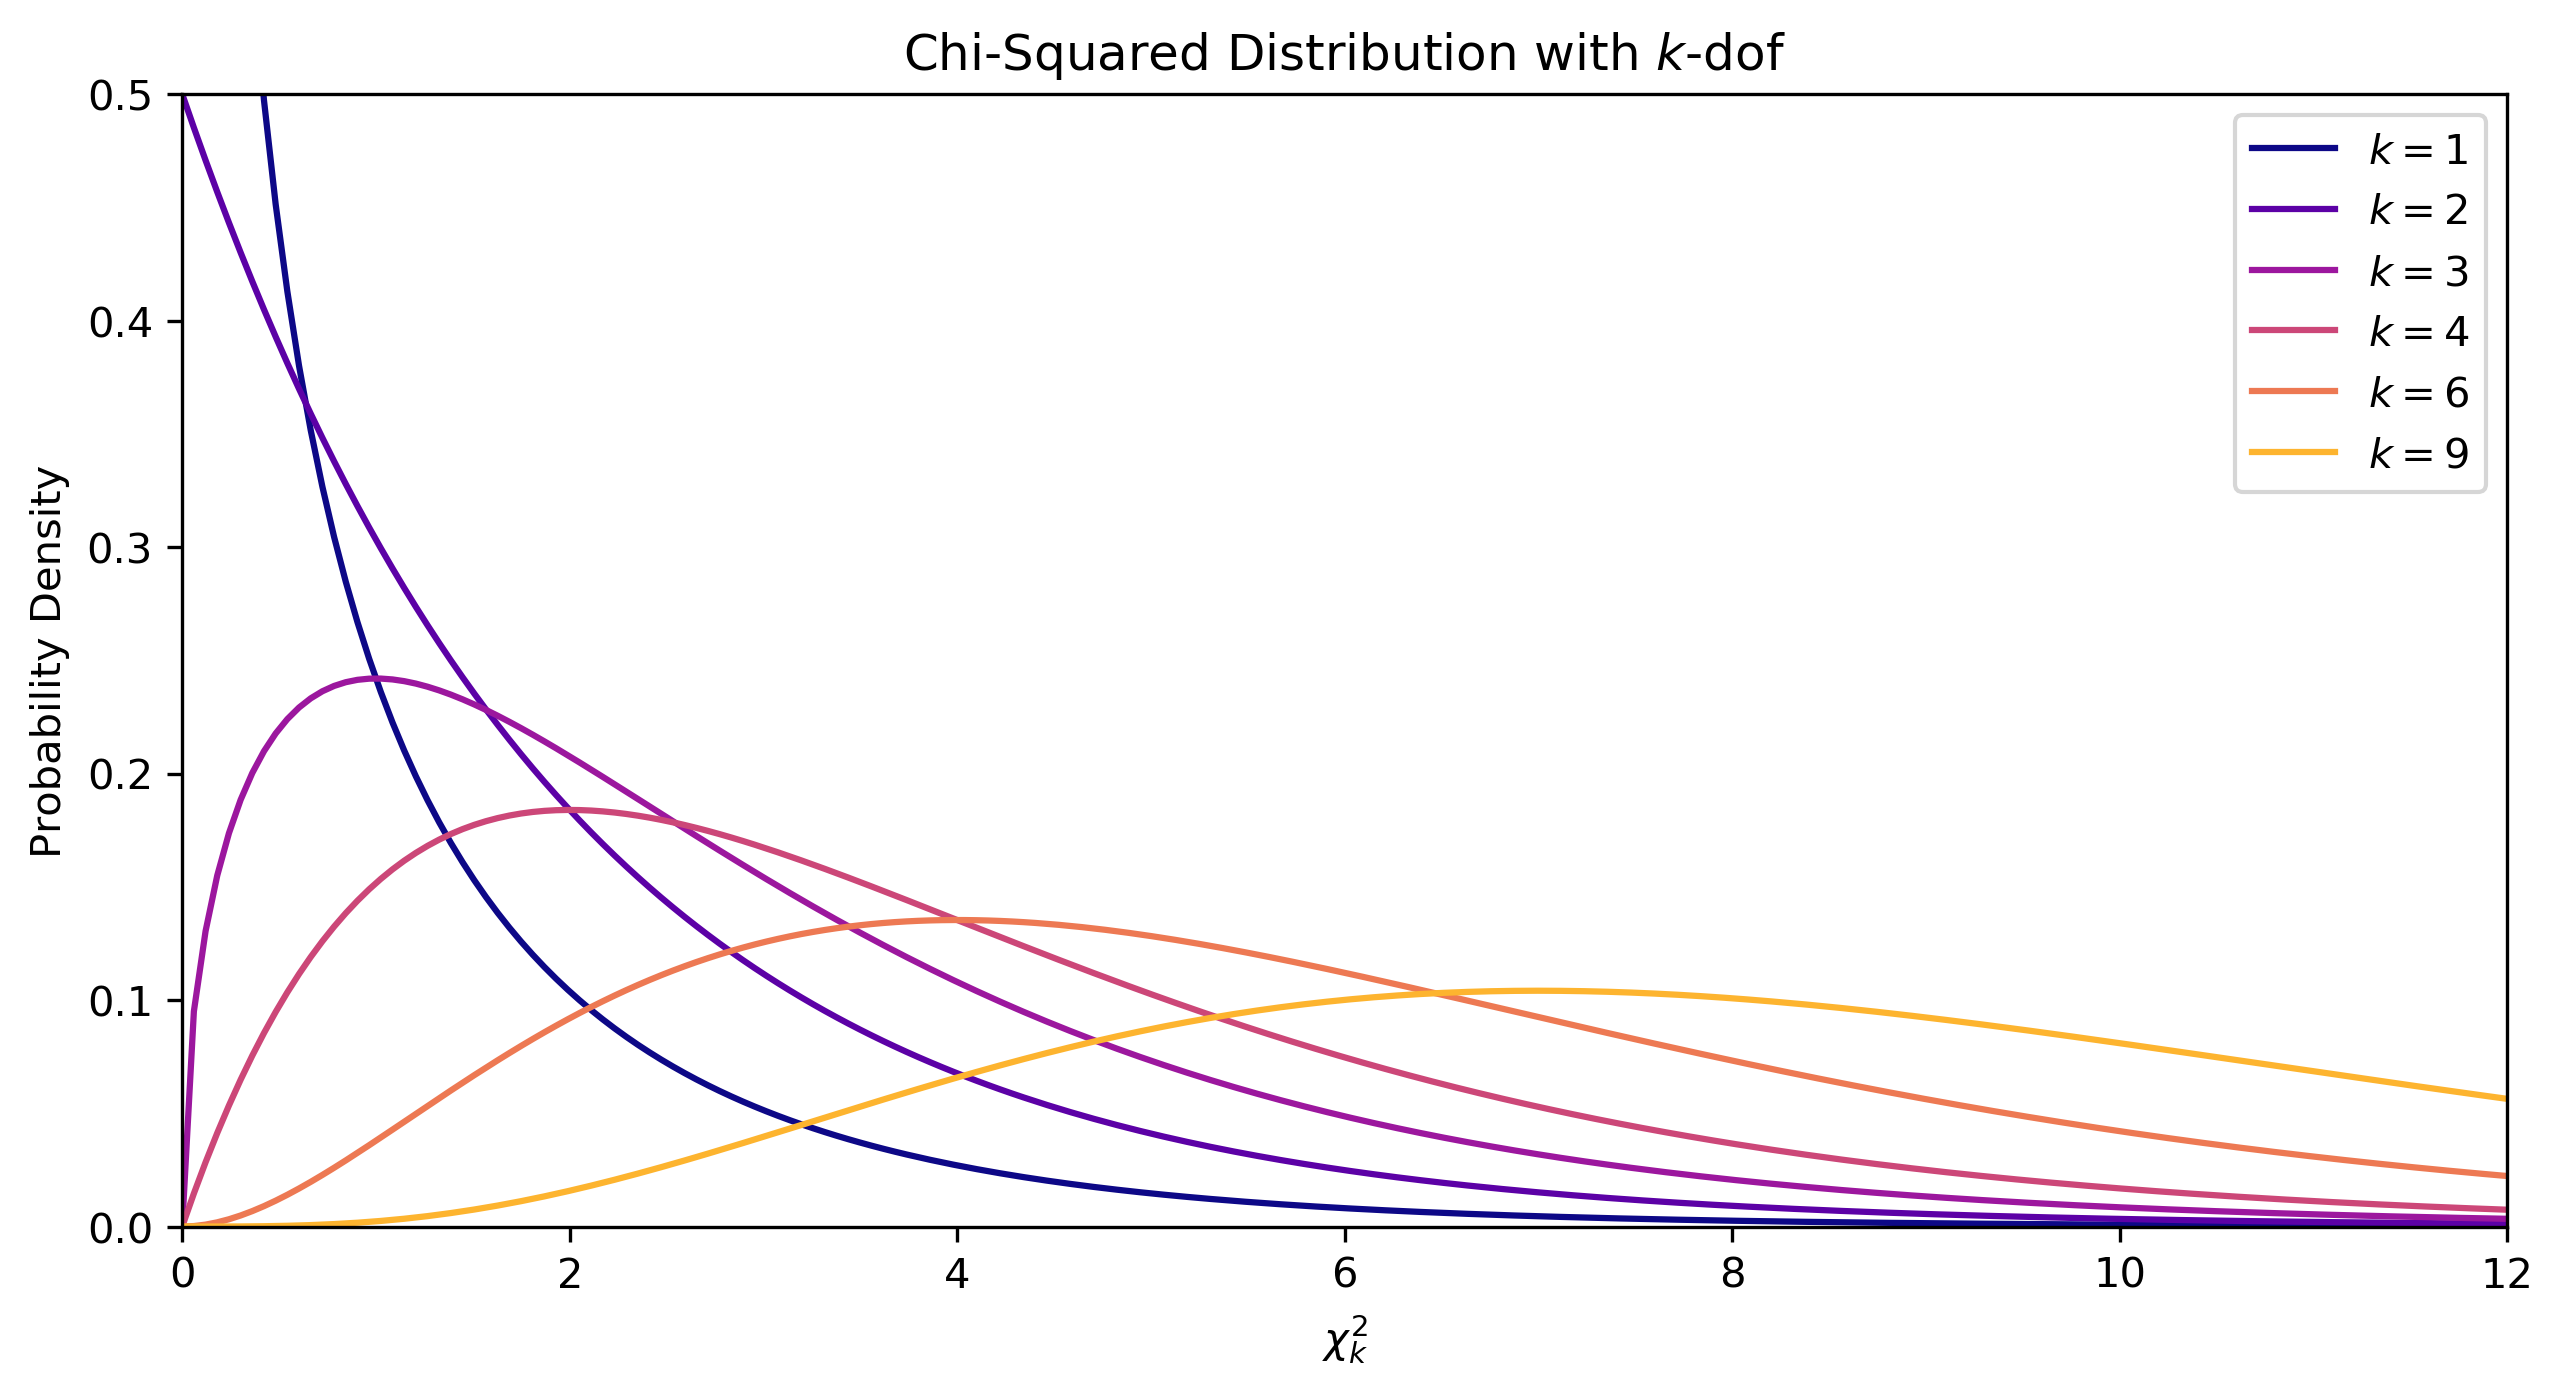
\includegraphics[width=11cm] {pdf}
\end{figure}

The distribution $ \chi^2_k $ has mean = $ k $ and variance = $ 2k $. The expectation value makes sense: $ E(\sum_i X_i) = \sum_i E(X_i) = k\cdot N(0,1)^2$ and the expectation value of the standard normal squared is 1.

\item UNCERTAINTY: the data that we collect has uncertainty, i.e. our data will have some amount of error. We assume that our measurments are normally distributed and that our uncertainty for a given point is the standard deviation. [NOTE: chi-squared analysis hold ONLY if errors are normally distributed]
\begin{figure}[H]
	\centering
	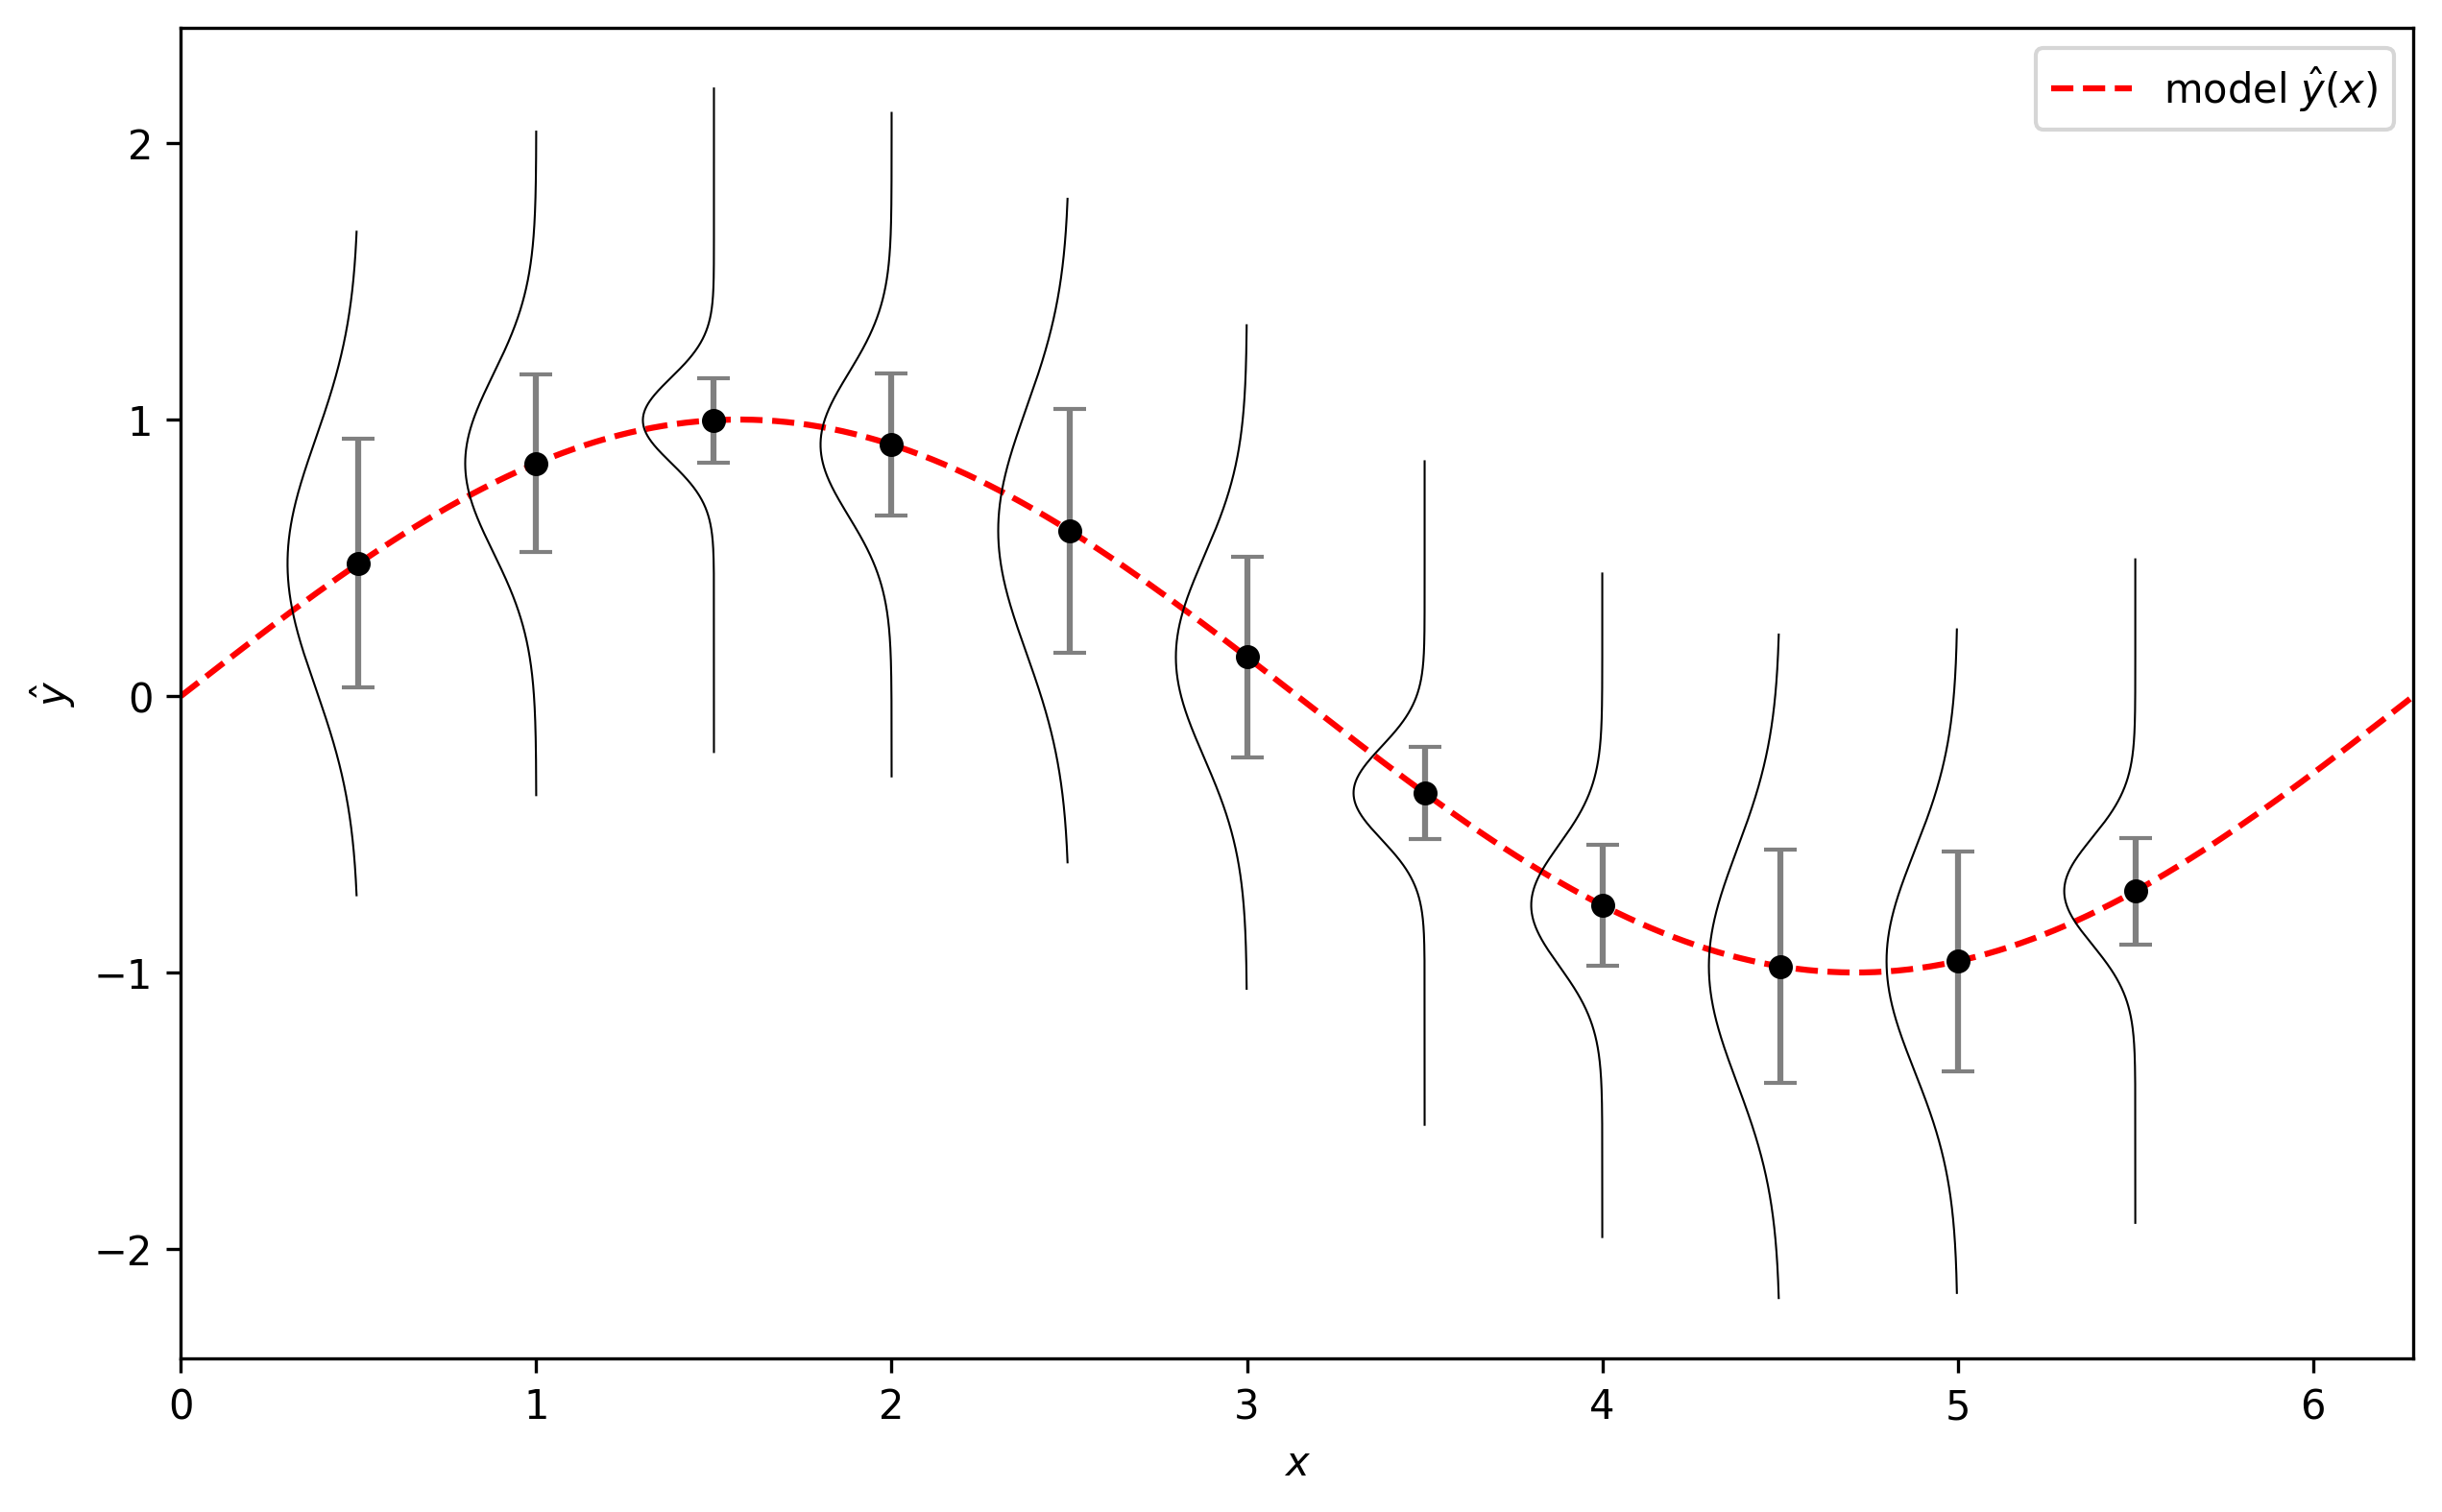
\includegraphics[width=11cm] {model}
\end{figure}
Then, for each $ x_i $, we measure $ y_i $ with uncertainty $ \sigma_i $, and,
\begin{equation}
	\frac{y_i - \hat{y}(\vec{a}, x_i) }{\sigma_i} \equiv X_i = N(0,1) 
\end{equation}

\item REDUCED CHI-SQUARED TEST: therefore,
\begin{equation}
	\sum_n 	\left(\frac{y_i - \hat{y}(\vec{a}, x_i) }{\sigma_i}\right)^2 = \sum_i X_i^2 = \chi^2_k
\end{equation}
This is the expression for the $ \chi^2 $ value for our data.

Q: For $ m $ data points and $ n $ fit parameters, how many dof are there? \textit{A: we will use $ m-n$ dof.} A hand-wavy argument is that there are $ m $ dof from the data points $ y_i $, but $ n $ constrains because we are minimizing the squares w.r.t the $ n $ parameters. Hence, a total of $ m-n $ dof. However, this is in general a tricky topic (see \href{https://arxiv.org/abs/1012.3754}{one interpretation}).
\begin{equation}
		\text{dof} = m-n
\end{equation}
The reduced chi-squared is,
\begin{equation}
		\boxed{ \chi^2_r = \frac{\chi^2_k}{k} = \frac{1}{\text{dof}}\sum_n 	\left(\frac{y_i - \hat{y}(\vec{a}, x_i) }{\sigma_i}\right)^2}
\end{equation}
The $ \chi^2_k $ distribution has mean $ k $, so we expect $ \chi^2_r $ to have mean $ 1 $. Isn't this a bit surprising?
\begin{enumerate}
	\item $ \chi^2_r \gg 1$: the residues are too large (bad model, incorrect fit parameters) or the uncertainty is too small (we underestimated the uncertainty our of data so even a good model will have a large $ \chi^2_r $).
	\item $ \chi^2_r \ll 1$: the residues are too small (over-fitted data, fitting noise) or the uncertainty is too large (we overestimated the uncertainty of our data so even a bad model will have a small $ \chi^2_r $).
	\item The ideal value of $ \chi^2_r $ is not 0, which corresponds to no residuals and a perfect fit. This is because $ \sigma_i $ is never 0, we EXPECT our measurements to deviate by a reasonable amount and not perfectly match our model. The value WE EXPECT of $\chi^2  $ is 1 per dof.
	\item RULE OF THUMB: a good fit has $ 0.8<\chi^2_r <1.5 $ (I couldn't trace where this comes from, but it's likely arbitrary to a certain extent)
\end{enumerate}

\begin{figure}[H]
	\centering
	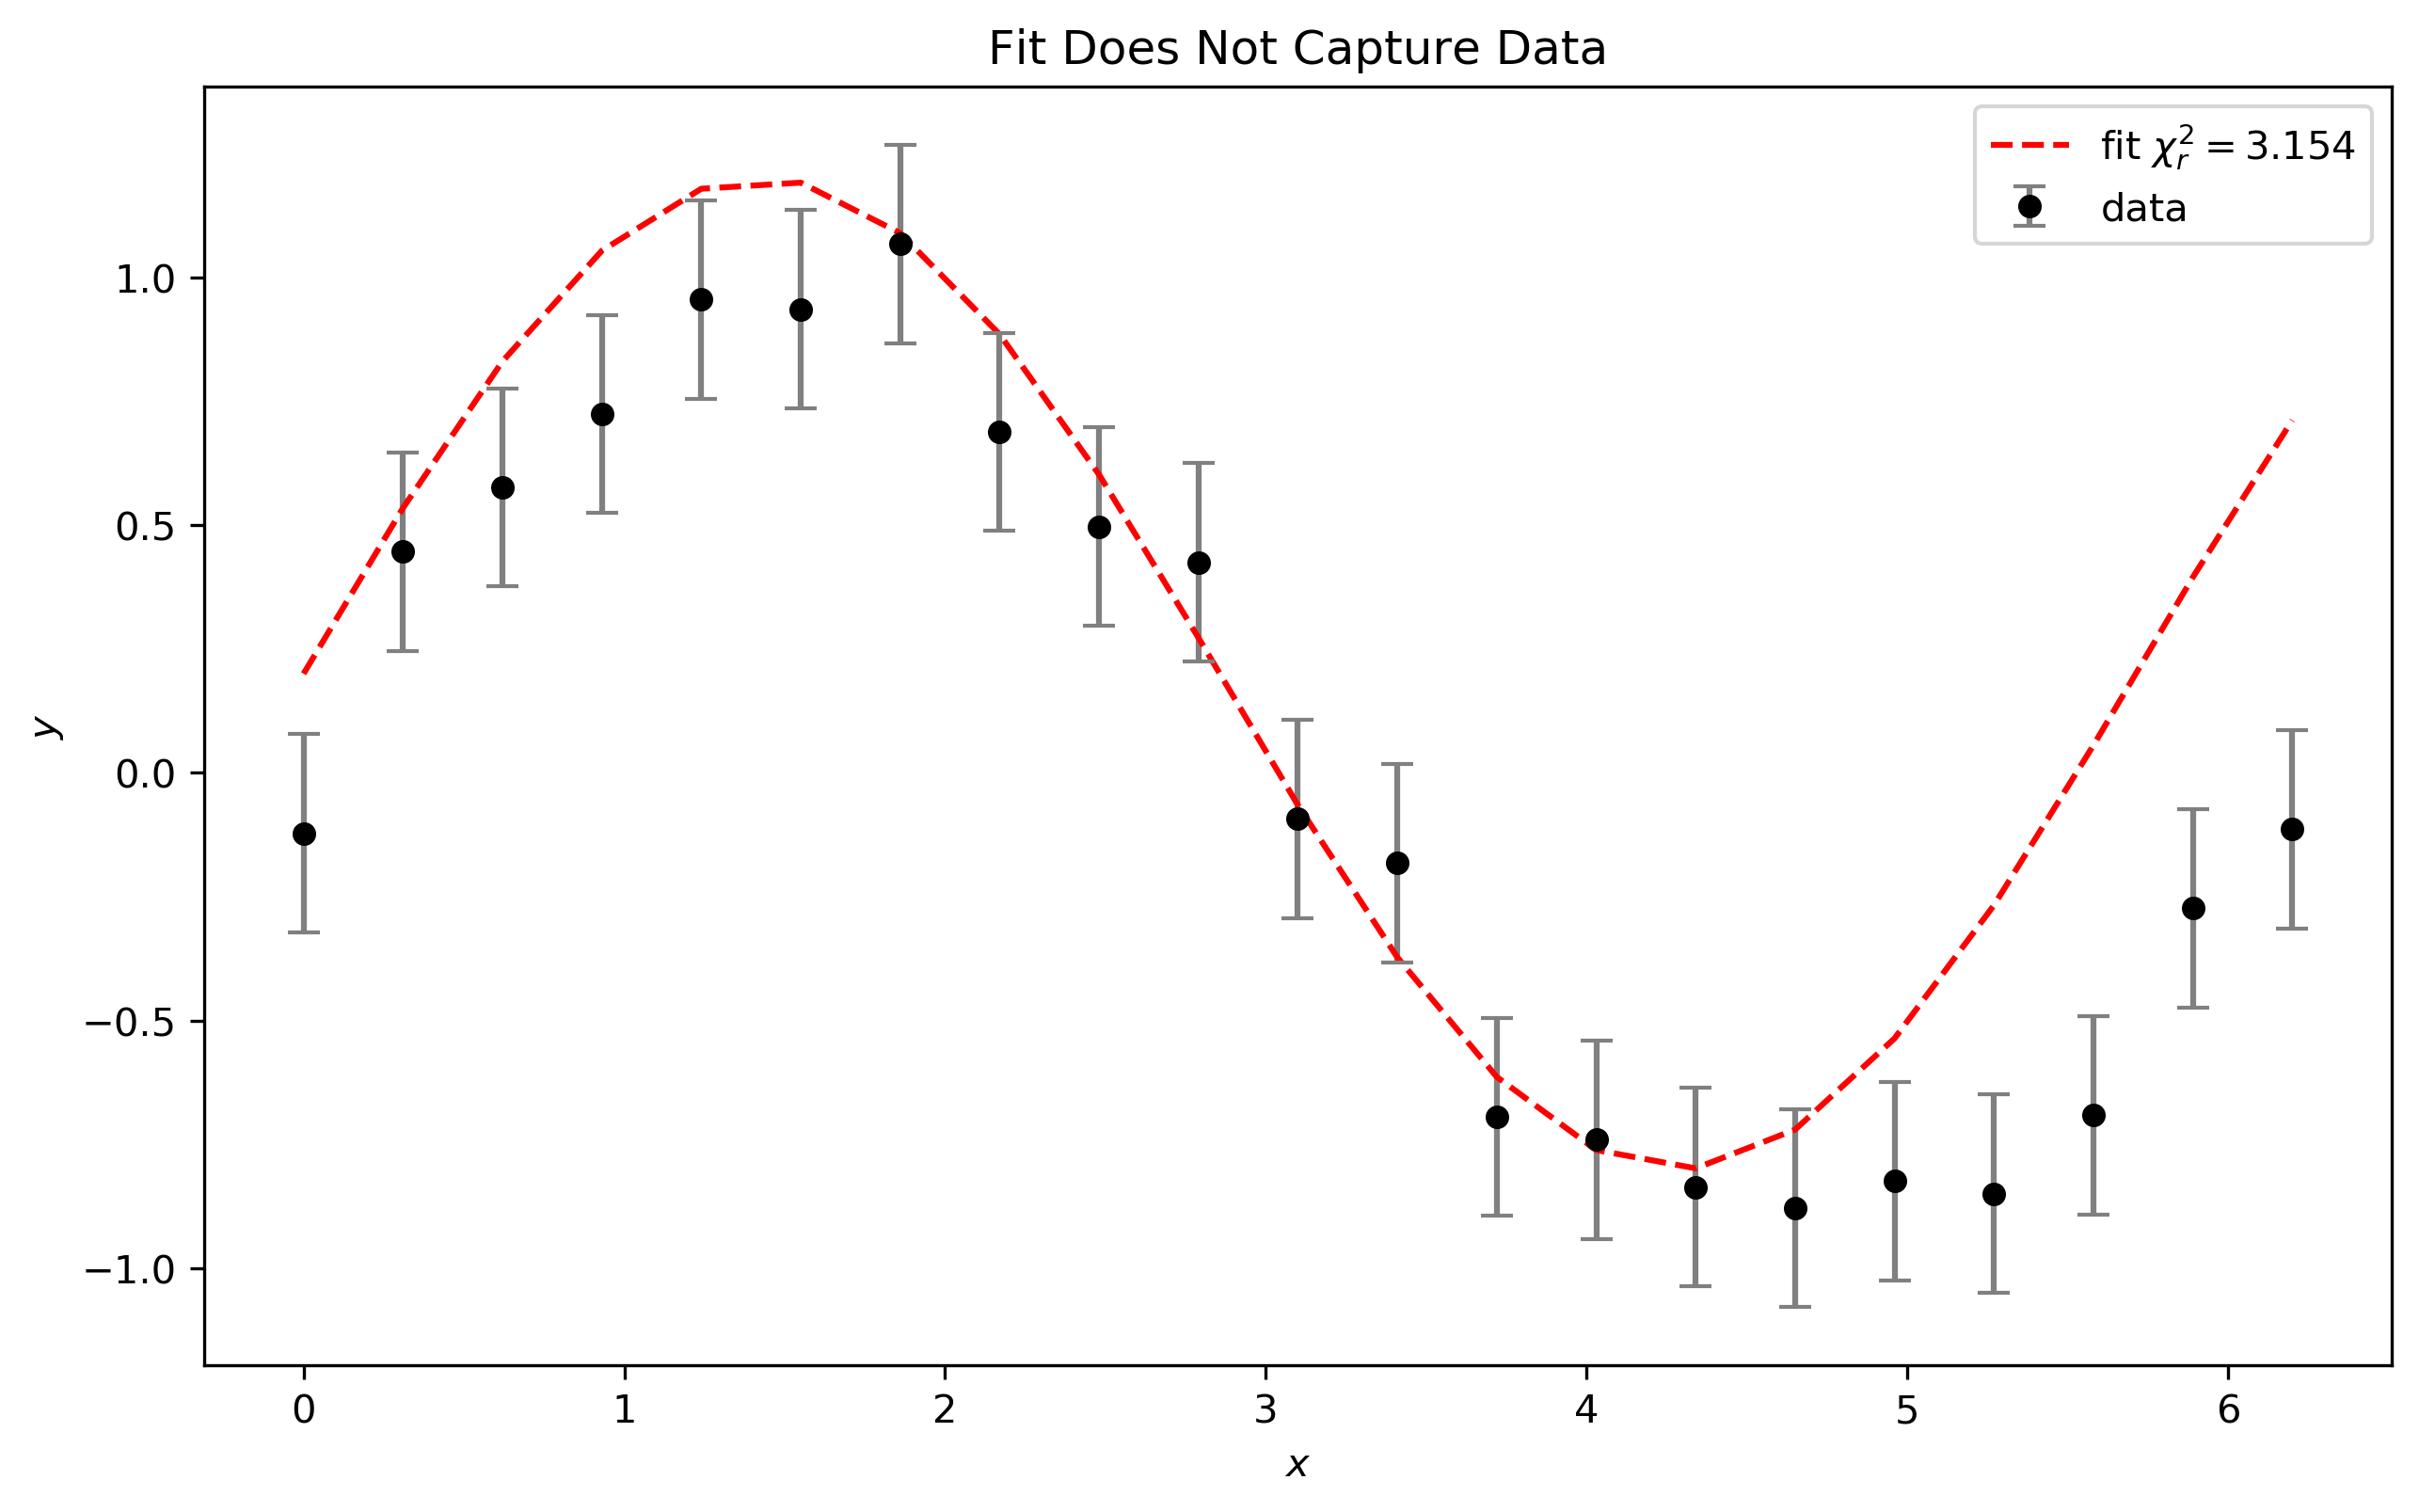
\includegraphics[width=11cm] {bad}
\end{figure}
\begin{figure}[H]
	\centering
	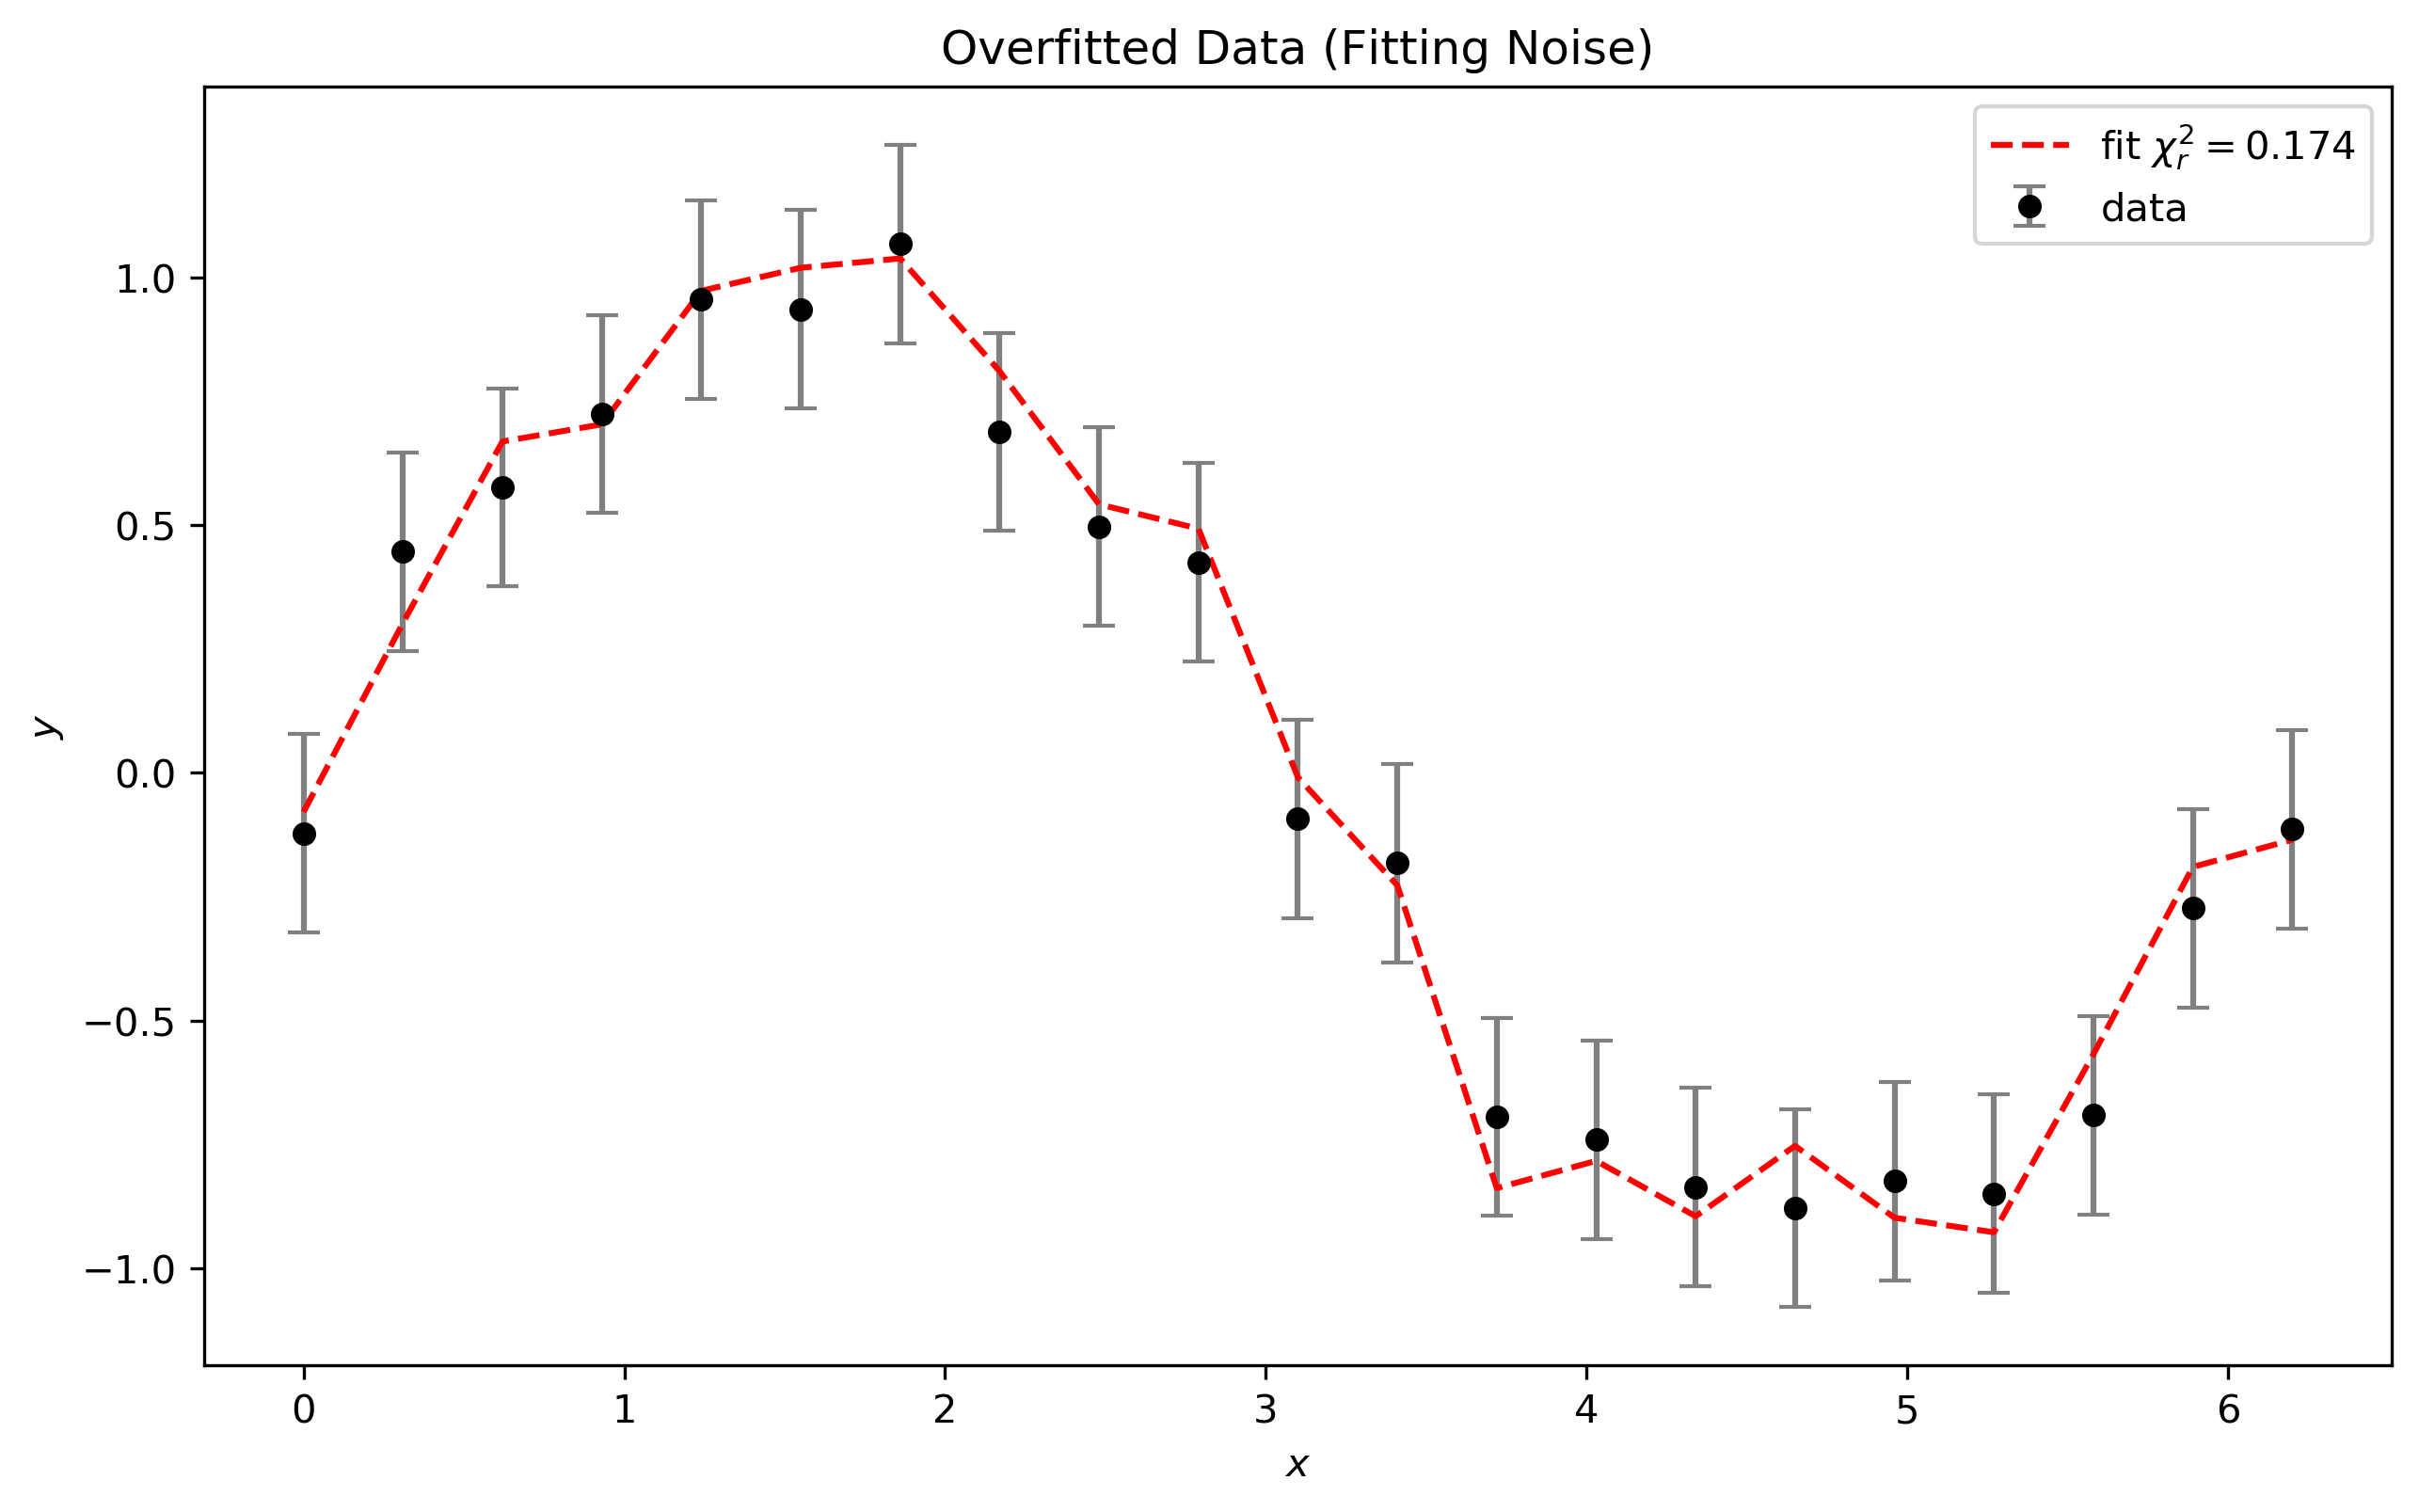
\includegraphics[width=11cm] {over}
\end{figure}
\begin{figure}[H]
	\centering
	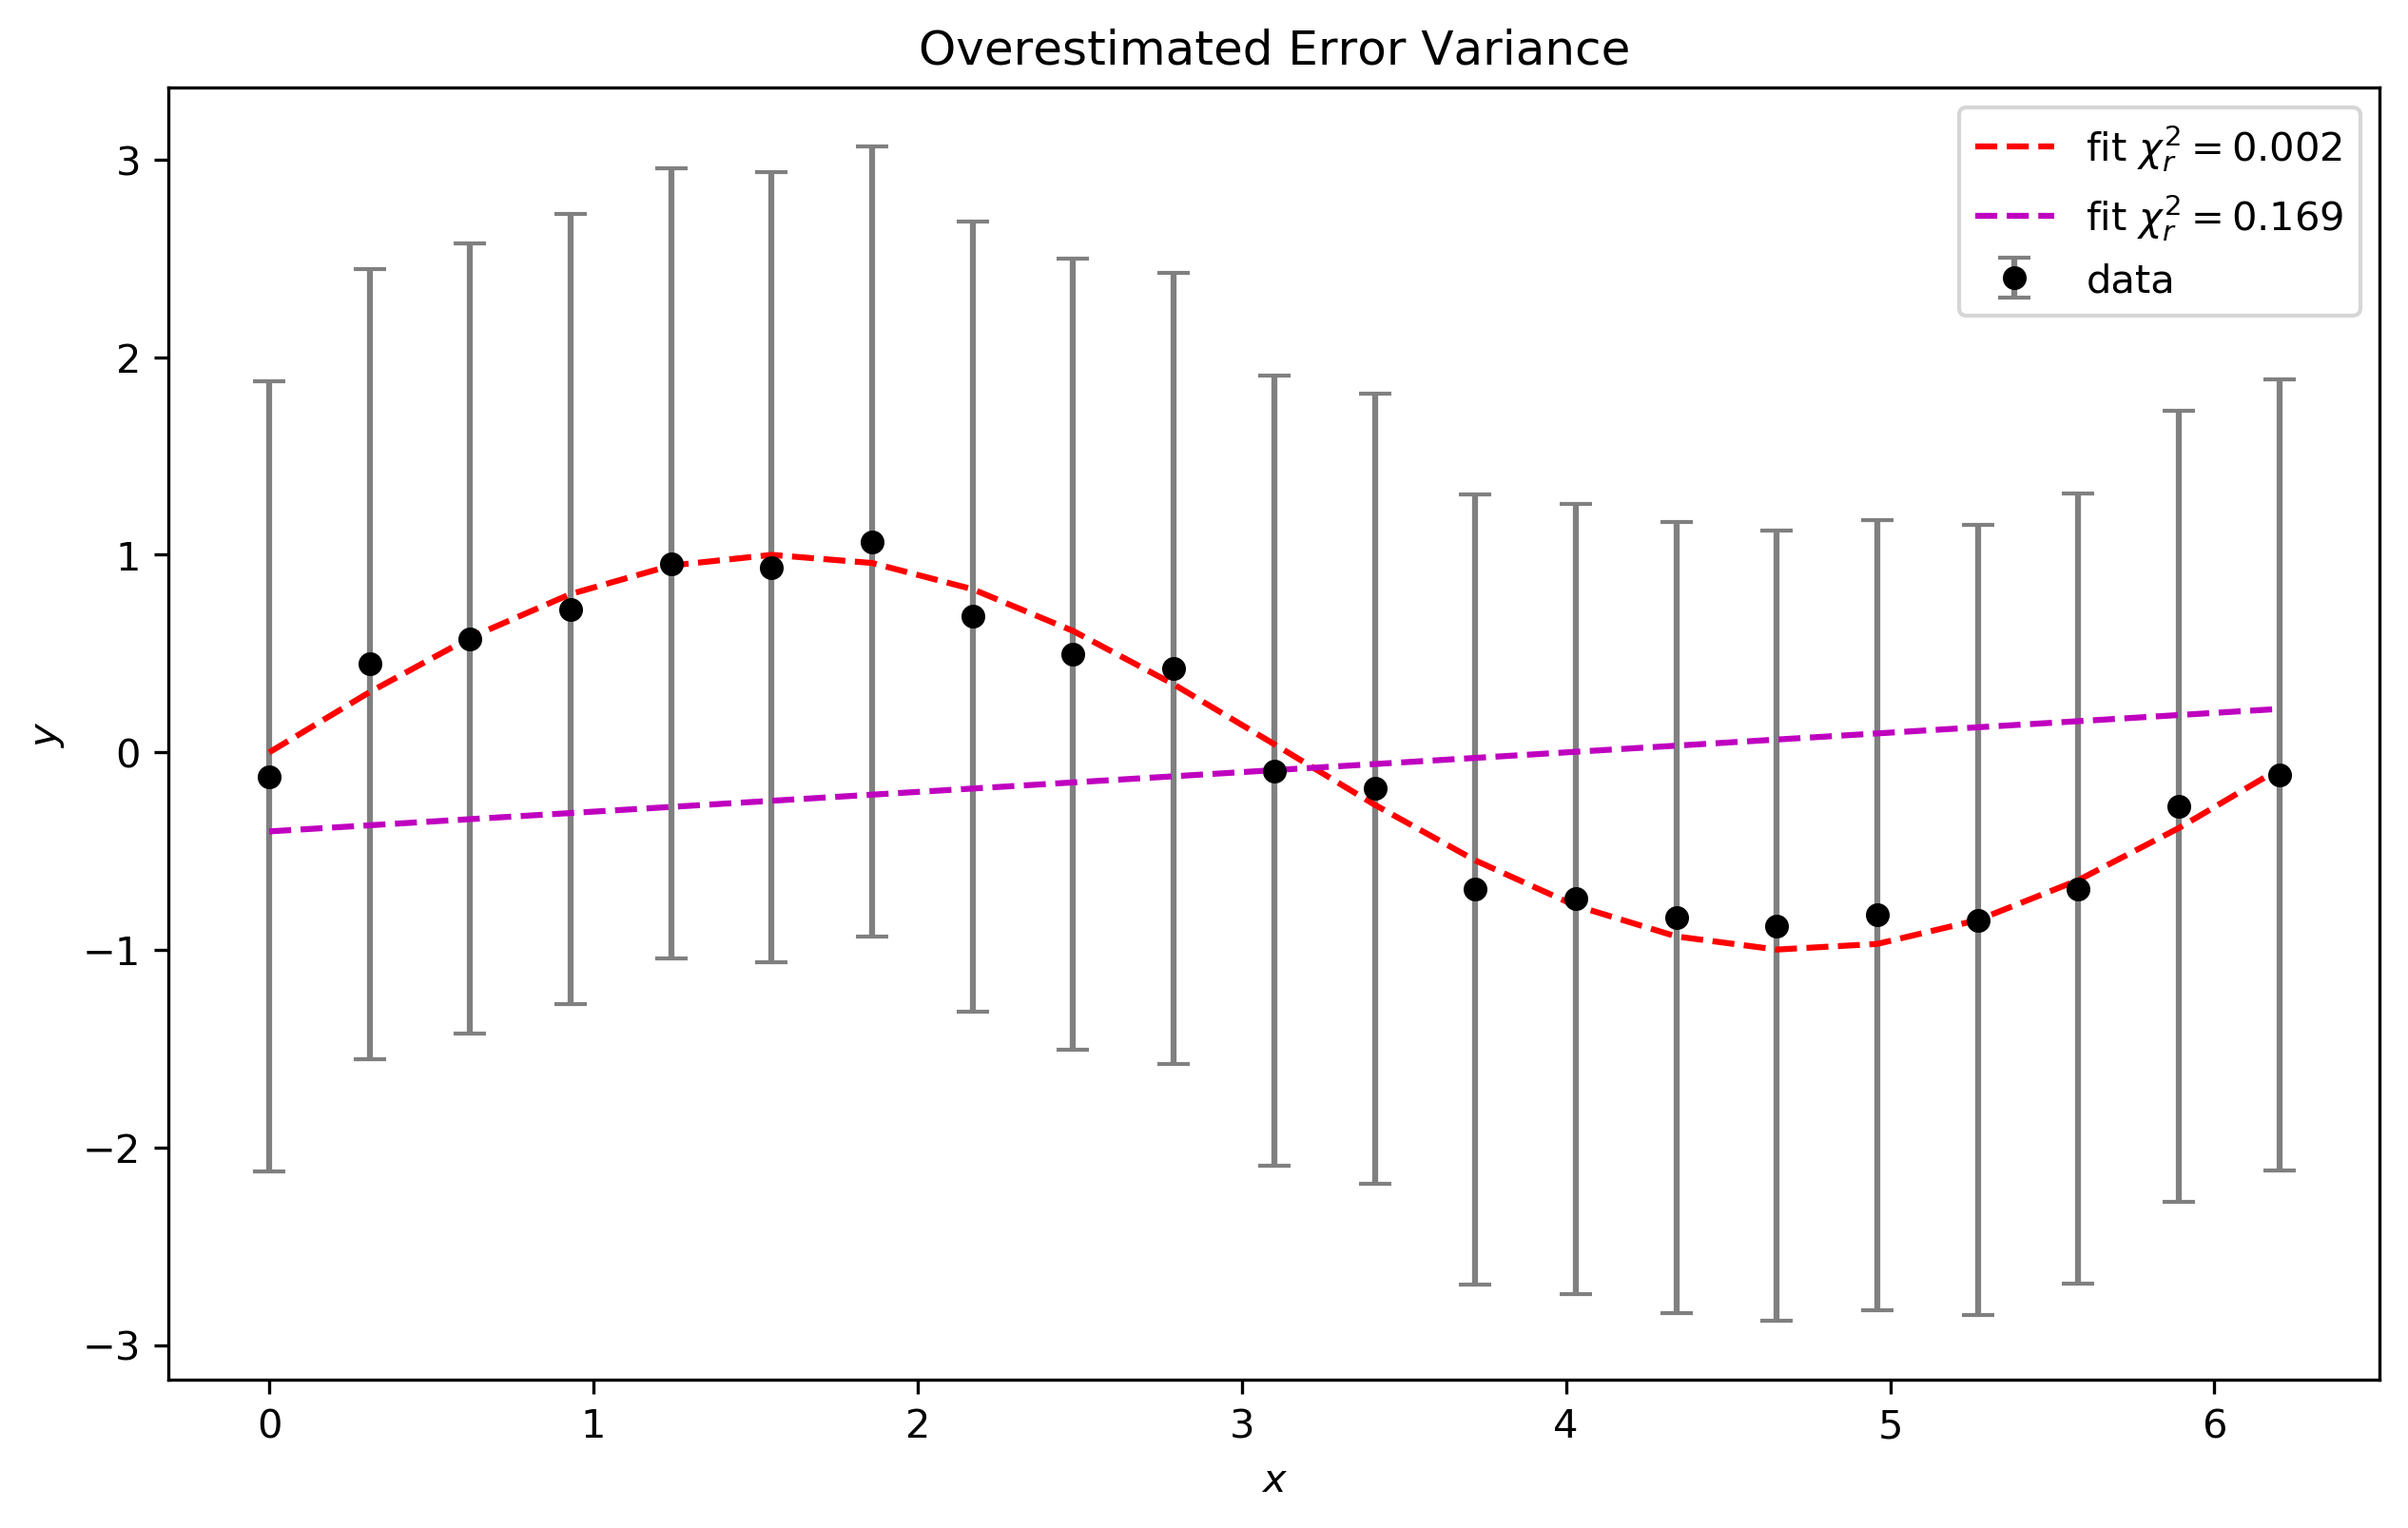
\includegraphics[width=11cm] {var}
\end{figure}

\end{itemize}

\section{Summary}
\begin{itemize}
	\item We discussed the least squares method, and it's implementation in python.
	\item We explained the reduced chi-squared distribution and it's usefulness in determining goodness-of-fit.
\end{itemize}

\end{document}
